\documentclass[10pt,a4paper]{article}
\usepackage[utf8]{inputenc}
\usepackage[parfill]{parskip}
\usepackage[section]{placeins}
\usepackage{graphicx}
\usepackage{array}
\usepackage{tikz}
\usepackage{apacite}
\usepackage{url}
\usepackage[left=3.00cm, right=3.00cm, top=3.00cm, bottom=3.00cm]{geometry}
%\usepackage[printwatermark]{xwatermark}
%\usepackage{xcolor}

%\newwatermark[allpages,color=red!40,angle=45,scale=4,xpos=0,ypos=0]{DRAFT}

\title{{\Huge Customer Experience Text Analytics for Social Media}}
\author{Christoph Emunds, Benedikt Heinrichs, Dominik Nerger, Richard Polzin}
\date{\today}

\begin{document}
	\maketitle
	
	\section{Introduction}
	The project presented in this project plan focusses on finding and analyzing customers' opinions on products and their aspects from social media posts.
	
	This project plan describes related work and the principals that we are going to build upon. We present the current state of the project explain what has been done so far. Finally, we define the goals for our project and give a schedule for the upcoming tasks. 
	
	\section{Related work}
		\subsection{Word embeddings}
		%Word vectors are numeric representations of words where similar words have similar vectors. Word vectors are often used as input to deep learning systems. This process is sometimes called pretraining.
		
		More concise than the \textit{bag of words} model with one-hot encoded vectors, which, depending on the amount of words in the vocabulary, have a huge dimensionality, while only one of the vector's components is set to 1 and the rest to 0. Such simple models also fail to incorporate meaning of and similarities between words. For example in the sentences
		\begin{quote}
			the cat got squashed in the garden on friday
		\end{quote}
		\begin{quote}
			the dog got flattened in the yard on monday
		\end{quote}
		simple language models do not capture the similarities between the word pairs \textit{cat/dog}, \textit{squashed/flattened}, \textit{garden/yard} and \textit{friday/monday}.
		
		Today, word embeddings are used in a lot of natural language processing (NLP) tasks.
		
		A famous example for the expressive power of word embeddings is the following:
		
		\begin{displaymath}
			king-man+woman \approx queen
		\end{displaymath}
		
		This equation shows that if one were to subtract the vector representation for the word \textit{man} from the vector for \textit{king} and add the vector for \textit{woman}, this would result in a point near to the vector for the word \textit{queen}.
		
		\begin{figure}[h]
			\centering
			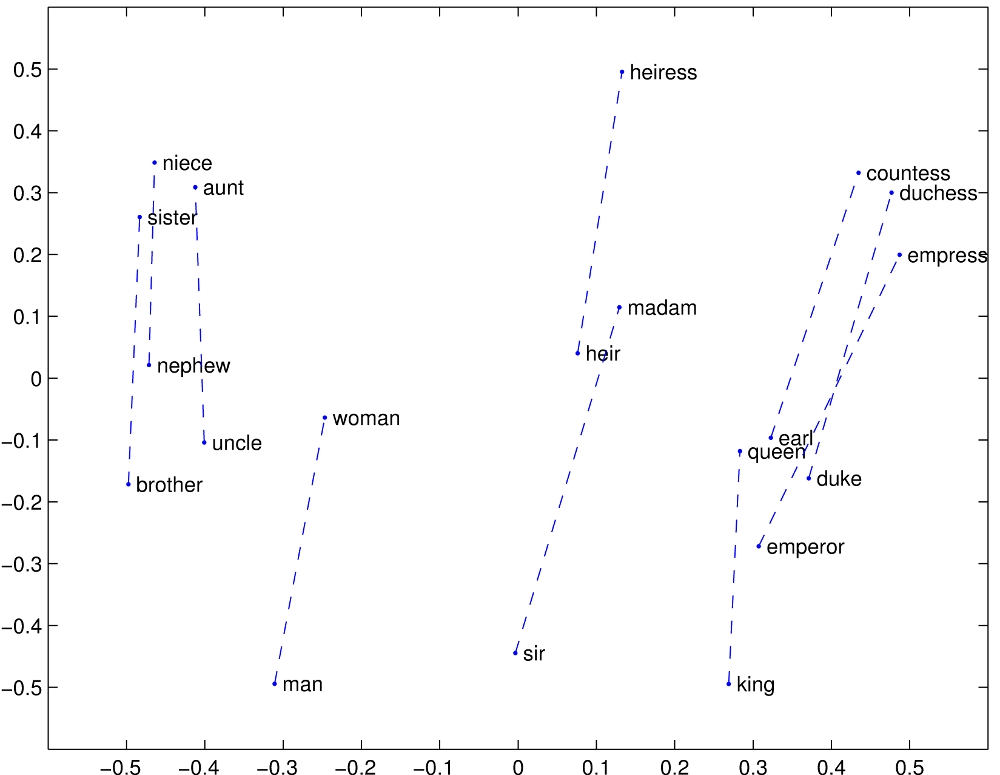
\includegraphics[width=0.8\linewidth]{data/man_woman}
			\caption{Representation of words relating to the differentiation between man and woman}
		\end{figure}
		
		The high dimensional vector representations of the words can be processed with the \textit{t-SNE} dimensionality reduction algorithm to be able to plot them in a two dimensional vector space.
		
		\subsection{POS-Tagging}

		POS-Tagging (part-of-speech tagging), also called grammatical tagging or word-category disambiguation, refers to the process of identifying partical parts of speech like nouns or verbs. 

		Identifying the role of a certain word within a sentence is important for the task of sentiment analysis, as identifying entities and their corresponding aspects can be handled much easier relying on certain assumptions about the part of speech of words.

		Frequent nouns or noun phrases often describe aspects of products and the vocabulary that is used to describe those usually converges. With such an approach many important aspects can easily be found, but on a more general scheme grammatic based relationships can be used to extract important aspects.

		For example words that express opinion on something, like 'great' or 'bad' can be incorporated in rules to extract aspects. To sum it up POS-Tagging is an important part of sentiment analysis.
		
		While being important POS-Tagging is also a complex problem. Word-forms in natural language are often ambiguous. For example the word 'dogs' in usually thought of as a plural noun, but can be used as a verb as well:

		\begin{quote}
			The sailor dogs the hatch.
		\end{quote}

		Due to the complexity machine learning techniques are often applied in POS-Taggers. Popular approaches such as the Viterbi algorithm, the Brill tagger or the Baum-Welch algorithm work with techniques such as dynamic programming, supervised learning or hidden markov models.
		
		\subsection{NER-Tagging}
		
		\subsection{Dependency parsing}
		
		Dependency parsing is a method of building up context in a sentence.
		It looks on the relations each word has with the other words and tries to create a meaning out of a sentence by that.
		
		For example the sentence "I saw a girl with a telescope" has two times the combination of an object with the word "a". 
		The word "girl" is specified by the verb "saw" and the object "telescope" is specified by the word "with" with references to the verb "saw". 
		The verb "saw" relates then to the noun "I" as it is the subject. 		
		A visualization can be seen in the following.
		This is however just one method of analyzing this sentence.
		Another way of seeing this sentence would be to relate the word "with" with the object "girl" which is possible in the language and gives the whole sentence a different meaning.
		
		\begin{figure}[h]
			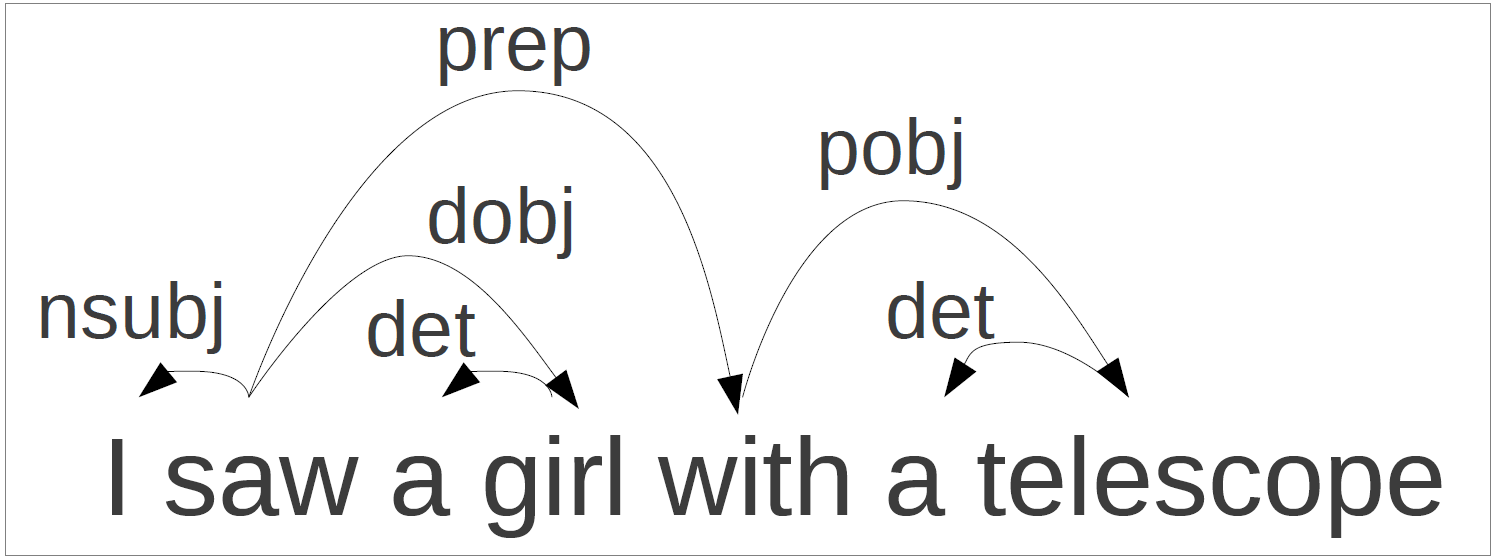
\includegraphics[width=\linewidth]{data/dependency}
			\caption{The dependency parsing example}
			\label{fig:dependency}
		\end{figure}
		
		This example has been taken from \cite{dependency}.
	
	\section{Extracting entities and aspects}
	
	Extract the posts' text into separate files.
	
	we will use a method proposed by Hu and Liu (2004) to extract entities and aspects.
	
	Annotate all files with POS-Tags.
	
	Identify frequent nouns and noun phrases with a POS-Tagger. Frequency threshold is chosen experimentally. People commenting on aspects of a product usually use a limited vocabulary. Thus, frequent nouns and noun phrases are most likely important aspects.
	
	However, since the first step can miss quite a lot of important aspects, the next step tries to find some of them by exploiting the relationships between aspects and opinion words.
	
	\section{Determining sentiment polarities}
	We will focus on two approaches
	
		\subsection{LSTM-Network}
		
		\subsection{Lexicon-based approach}
		lexicon-based approach, because it is unsupervised and generally more powerful than supervised learning(?)
		
		We will apply a method by Ding, Liu and Yu (2008), which has the following steps: First, all sentiment words and phrases in the text will be marked with the help of a sentiment lexicon.
		
		Second, sentiment shifters will be applied.
		
		Third, but-clauses must be handled.
		
		Fourth, opinions need to be aggregated.
	
		This method can be made more effective by applying dependency parsing to the sentences, such that the scope of each individual sentiment word can be determined more accurately. This allows us to discover the sentiment orientation of context dependent words (Bing Liu, 2012).

	\section{State of the project}
	We built and tested the syntax parser \textit{Parsey McParseface} (aka SyntaxNet) by Google, which we will use as POS-Tagger for extracting entities and aspects, because it is easy to use and yields state-of-the art results. Moreover, it is based on Google's Deep Learning Framework TensorFlow and therefore integrates nicely into the rest of our implementation.
	
	Use pre-trained word embeddings from the GloVe project.
	
	We preprocessed the data by extracting the actual text of the posts into separate files, which can be processed by SyntaxNet.
	
	We will utilize the sentiment lexicon by Bing Liu, which includes mis-spellings, morphological variants, slang and social-media mark-up of 2006 positive and 4783 negative words.
	
	\begin{table}[h]
		\centering
		\caption{Per-token accuracy of different POS-Taggers}
		\label{tab:posaccuracy}
		\begin{tabular}{|l|l|l|l|}
			\hline
			Model & News & Web & Questions \\
			\hline
			Ling et al. (2015) & 97.44 & 94.03 & 96.18 \\
			\hline
			Andor et al. (2016) & 97.77 & 94.80 & 96.86 \\
			\hline
			Parsey McParseface & 97.52 & 94.24 & 96.45 \\
			\hline
		\end{tabular}
	\end{table}
	
	\begin{table}[h]
		\centering
		\caption{Accuracy of different dependency parsers}
		\label{tab:parseraccuracy}
		\begin{tabular}{|l|l|l|l|}
			\hline
			Model & News & Web & Questions \\
			\hline
			Martins et al. (2013) & 93.10 & 88.23 & 94.21 \\
			\hline
			Zhang and McDonald (2014) & 93.32 & 88.65 & 93.37 \\
			\hline
			Weiss et al. (2015) & 93.91 & 89.29 & 94.17 \\
			\hline
			Andor et al. (2016) & 94.44 & 90.17 & 95.40 \\
			\hline
			Parsey McParseface & 94.15 & 89.98 & 94.77 \\
			\hline
		\end{tabular}
	\end{table}

	\section{Goals and schedule}
	The overall goal is to extract as many quintuples $(e_i, a_{ij}, s_{ijkl}, h_k, t_l)$ as possible, where $e_i$ is the $i$'th entity, $a_{ij}$ is the $j$'th aspect of entity $i$ the opinion is expressed on, $s_{ijkl}$ is the sentiment polarity, $h_k$ the opinion holder and $t_l$ the time at which the opinion was expressed.
	
	Build a database with opinions and statistics on products and their aspects.
	Visualization via dashboard.

	\newpage

	\nocite{DBLP:journals/corr/AndorAWSPGPC16}
	\nocite{Liu12sentimentanalysis}
	\nocite{Zhang2014}
	\nocite{pennington2014glove}
	\nocite{syntaxnet}
	\nocite{Ding:2008:HLA:1341531.1341561}
	\nocite{Hu:2004:MSC:1014052.1014073}

	\bibliography{rp}
	\bibliographystyle{apacite}
\end{document}